\chapter{Testing \& Results}
This chapter details the testing that was carried out to assess the performance of different parts of the system, such as the human detection and direction, as well as the powered wheelchair and Hololens system as a whole. We outline the test setups used to evaluate the performance of the systems, as well as the results of the tests and what they imply about the implemented system.

\section{Human Detection and Distance}
This section is concerned with testing the Human Detection \& Direction system and the Hologram GameObject placement. To ensure the system will be able to detect real people moving around in the surroundings, it is necessary to test the system detecting people at different distances and the directions they are facing. We also want to test the accuracy of the spatial mapping system in terms of correcting the real world positions of the GameObjects representing the detected people. We utilize the Microsoft Hololens and the HDD system for this test.

\subsection{System Description} \label{sec:hddSys}
As explained in the Implementation chapter of this report, the front facing camera uses ROS topics to stream video frames to a partner computer the HDD system is implemented on. The HDD processes the frames and detects people and determines whether they are facing the PWU or not. The bounding box of the detections and directions are sent back to the Unity application. Initially, the application converts the pixel co-ordinates of the detections to corresponding world co-ordinates. We then use the spatial mapping and ray casting capabilities of the Hololens to correct the world position distances of the holograms representing the detected people.

\subsection{Test Setup} \label{sec:testSetup}
We setup a testing ground in the ICRS Lab on the 5th floor of the EEE building. We marked out points at 1 meter intervals which indicate where the target people should stand. We asked the person wearing the Hololens to sit down in a chair to emulate the position and height a PWU would be at when sitting in the wheelchair. Figure \ref{fig:hddTestSetup} shows the experimental setup in the lab. For this step, all subjects were stationary, except when the target person moves between the markings.

\begin{figure}[ht]
	\centering
	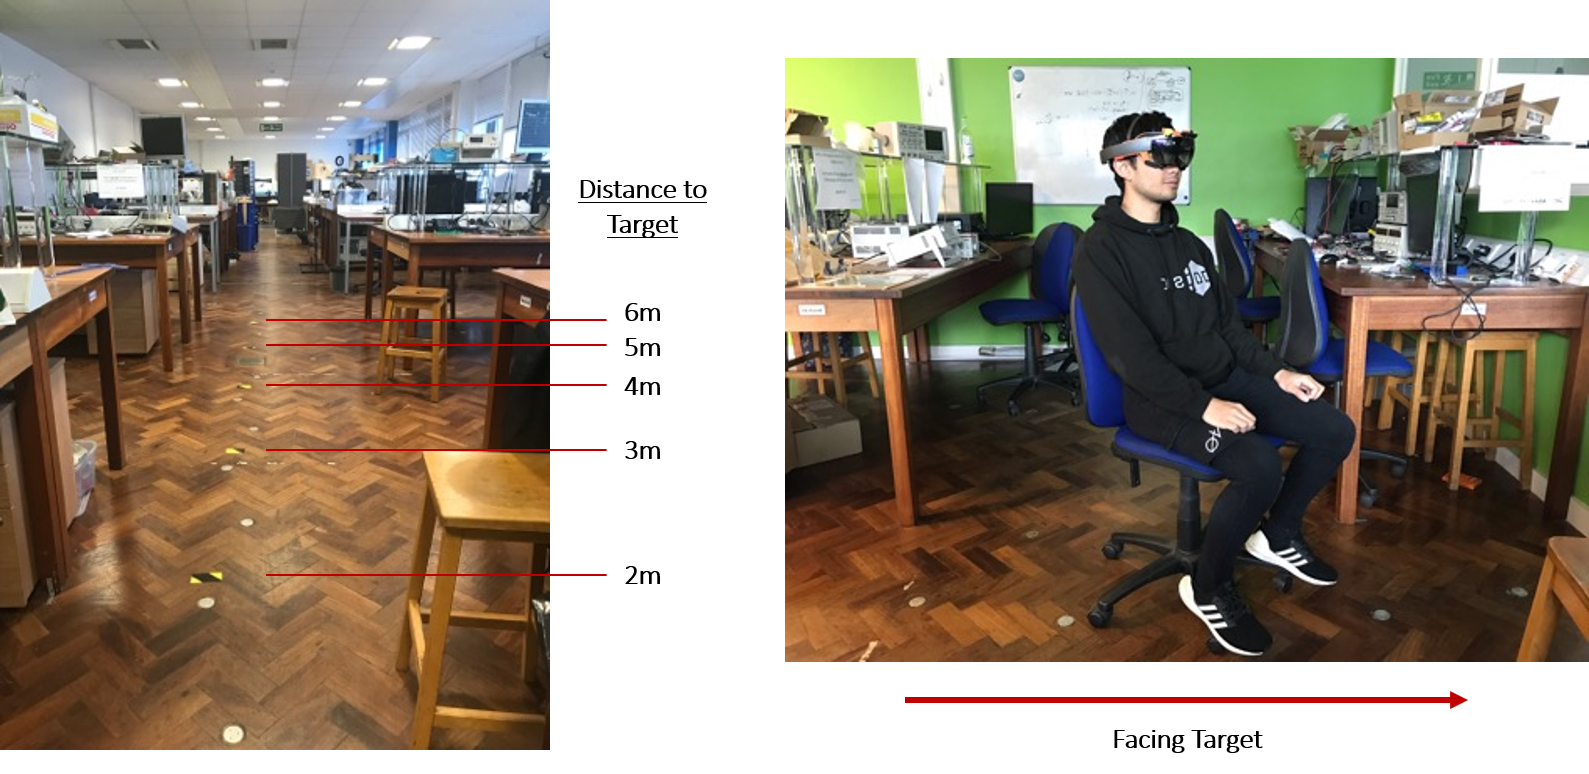
\includegraphics[width=1.0\linewidth]{img/chapter6_test/hddTestSetup.png}
	\caption{The experimental setup used to test the HDD and Hololens spatial mapping accuracy. We asked the people acting as targets to stand at 1 meter intervals while a person sitting down wearing the Hololens looked at them using the front facing camera.}
	\label{fig:hddTestSetup}
\end{figure}
 
We modified the Hololens Unity application to display holograms showing the distance between the Hololens and the target person in meters. We asked the person wearing the Hololens to call out the value the hologram displayed as the target person stood at different markings. To verify the readings, we recorded the Hololens display using the Windows Device Portal and watched them over after the test. Recording the hololens view also allowed us to see how the distance reading change as the target person moves.
 
\subsection{Test Procedure}
We asked three different people to sit in the chair and wear the Hololens. Before commencing the test, we allowed the people to learn how to wear the Hololens properly, ensuring the Hololens was correctly placed on the bridge of the users nose. We also allowed them to do several test detections to familiarise them with how the distance holograms would be rendered. This was done so that each participant would be able to detect the target person and call out the distance displayed by the hologram.

\paragraph{} The selected people all had different amounts of experience with the Hololens. One user was a complete novice, putting the Hololens on for the first time to participate in the test. One was an intermediate, having worn the Hololens a few times during the development of this project and the last person was more experienced with the Hololens and how the HDD system would detect the target people.

\paragraph{} We asked the target person to face forward at each marker, before turning their back and facing away from the Hololens user. This was done to check if there were any differences between the placement accuracy of the GameObjects for different orientations of the person.

\subsection{Results}
We show the results of the experiment in Figure \ref{fig:hddResults}, which compares the accuracy of hologram placement after spatial mapping and ray casting with the true world position of the detected person. Each test subject was given several seconds to adjust their head positions to ensure a detection was achieved. Despite this, none of the three test subjects were able to get holographic distances for a target at $6$m or further. This may indicate that the system was unable to detect a person at that distance, but what is more likely  is that the spatial mapping of the Hololens was unable to detect a surface that far away to render the distance hologram on. By looking at the debug log messages in Visual Studio 2017, we verified that there were indeed detections at $6$m, but they returned inaccurate values distance values.

\begin{figure}[ht]
	\centering
	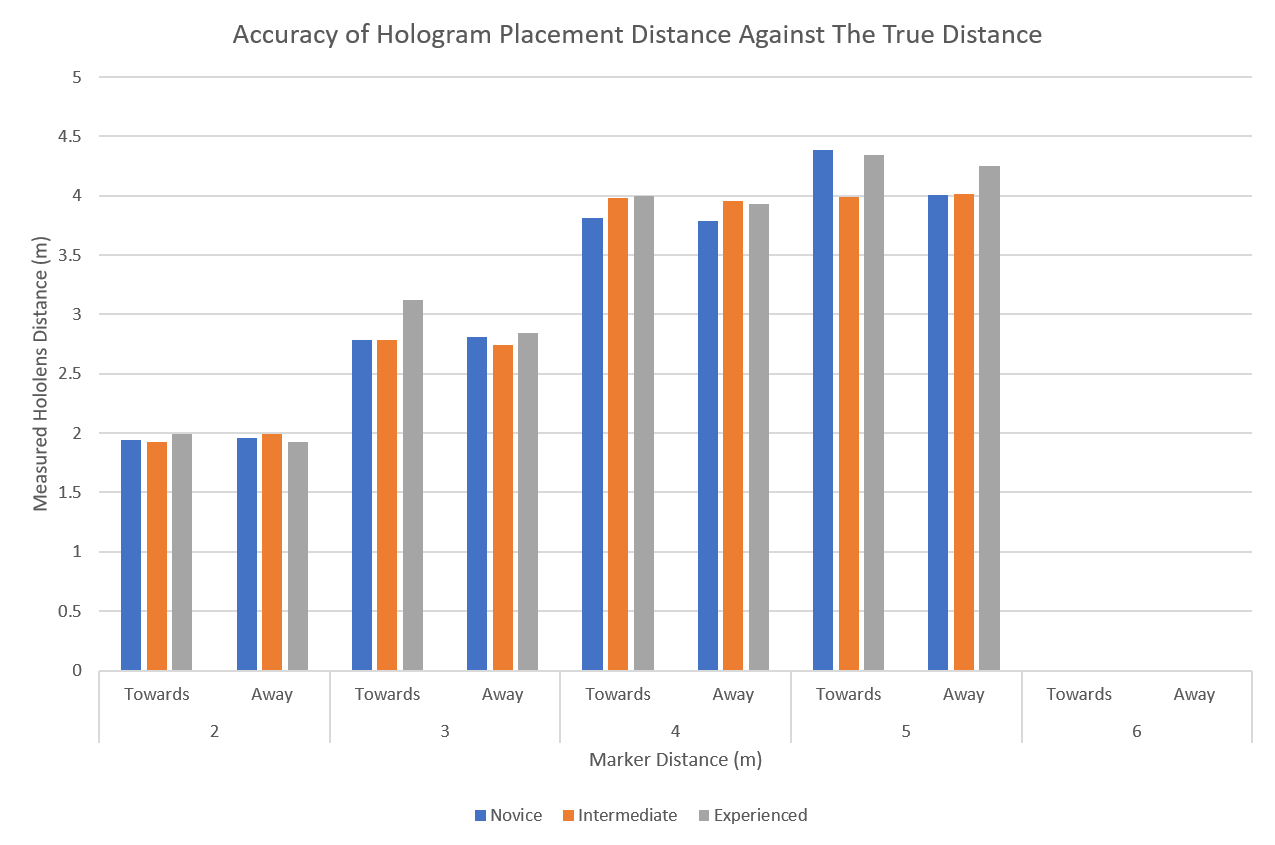
\includegraphics[width=1.0\linewidth]{img/chapter6_test/hddtestresults.png}
	\caption{The graph shows that there is no significant difference between the orientation of the target. We note the decrease in accuracy past $4$m, and the lack of holograms at $6$m.}
	\label{fig:hddResults}
\end{figure}

The data shows that there is no significant difference in hologram placement distance for target persons facing towards or away from the Hololens. However, we note that the hologram placement accuracy decreases the further away the target person is from the Hololens. This is further shown from the Hololens view recordings in Figure \ref{fig:marek}, whereby we can see that the placement of the hologram is not on the target person, but a surface just behind the target.

\begin{figure}[ht]
	\begin{subfigure}[b]{.32\textwidth}
		\centering
		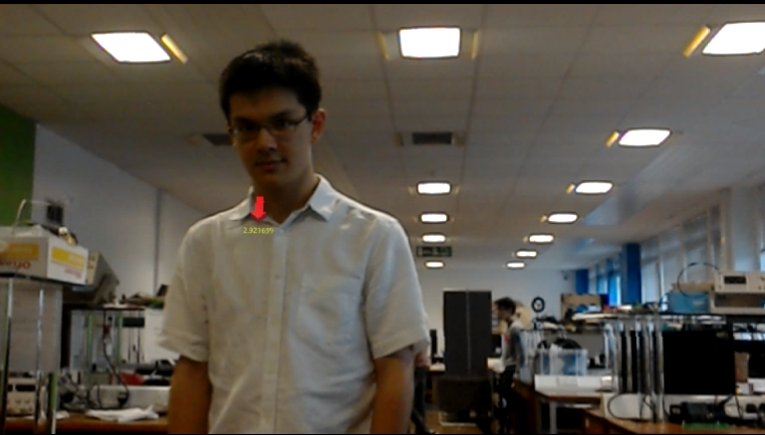
\includegraphics[width=1.0\linewidth]{img/chapter6_test/marek.png}
		\caption{Subject at 2m}
	\end{subfigure}%
	\hspace{\fill} 
	\begin{subfigure}[b]{.32\textwidth}
		\centering
		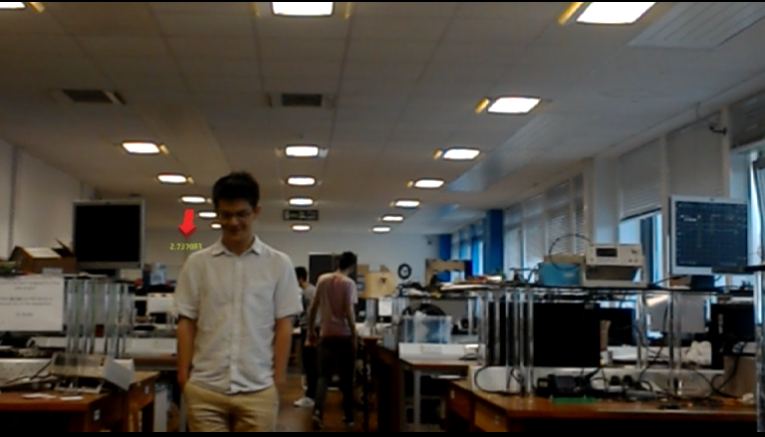
\includegraphics[width=1.0\linewidth]{img/chapter6_test/marek1.png}
		\caption{Subject at 3m}
	\end{subfigure}
	\hspace{\fill} 
	\begin{subfigure}[b]{.32\textwidth}
		\centering
		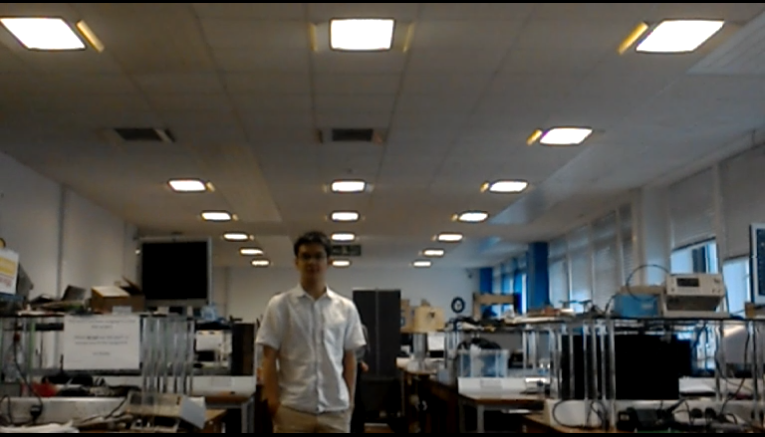
\includegraphics[width=1.0\linewidth]{img/chapter6_test/marek2.png}
		\caption{Subject at 6m}
	\end{subfigure}
	\vspace{-1\baselineskip}
	\begin{center}
		\caption{Target person at different distances viewed through the front-camera of the Hololens. We note that the accuracy of the hologram placement decreases as the target is further away.}
		\label{fig:marek}
	\end{center}
	\vspace{-2\baselineskip}
\end{figure}

\paragraph{} After the test, we asked the test subjects on qualitative feedback on how easy it it is to view a hologram. As expected, the novice Hololens user had difficulty seeing holograms due to the limited FOV of the device. The novice stated that the holograms were being rendered too high up, as they could only see the bottom of the hologram, as the rest of it was slightly out of view unless they tilted their head upwards. The intermediate user had a similar experience, but only had difficulty in seeing the holograms when the target person was closer than 2 meters.

\section{Gazebo Simulation}
Before testing the system using ARTA in the real world, we used the robot simulation tool Gazebo to test how the reactive control system would manipulate the ARTA control signals in response to person detections at different distances. The purpose of this simulation is to test the communication between ARTA and the Hololens, and how the reactive control system manipulates the velocity of the wheelchair as it approaches a detected person. We also want to test if the system can decide if the detections are to the side of the wheelchair or in front, and react appropriately. 

\subsection{System Description}
For this test, we use the same system as the one described in Section \ref{sec:hddSys}, with the addition of the Gazebo simulation of the ARTA powered wheelchair. We communicate the ARTA control signals to the Hololens, which checks the trajectory of the wheelchair and determines if a collision with a detected person is imminent. If the reactive control system decides a detected person is a collision risk, it reduces the velocity of the wheelchair in order to avoid a collision.

\subsection{Test Setup}

\subsubsection{Gazebo Simulation}
We use the Gazebo Simulation software to load a world built using the height map for the hallway outside the Personal Robotics Lab on the 10th floor. We then load the Unified Robot Description Format (URDF) model of ARTA into the world and run the ROS nodes controlling the powered wheelchair. We control the simulated wheelchair using the keyboard on the computer instead of a joystick.

\begin{figure}[ht]
	\begin{subfigure}[b]{.48\textwidth}
		\centering
		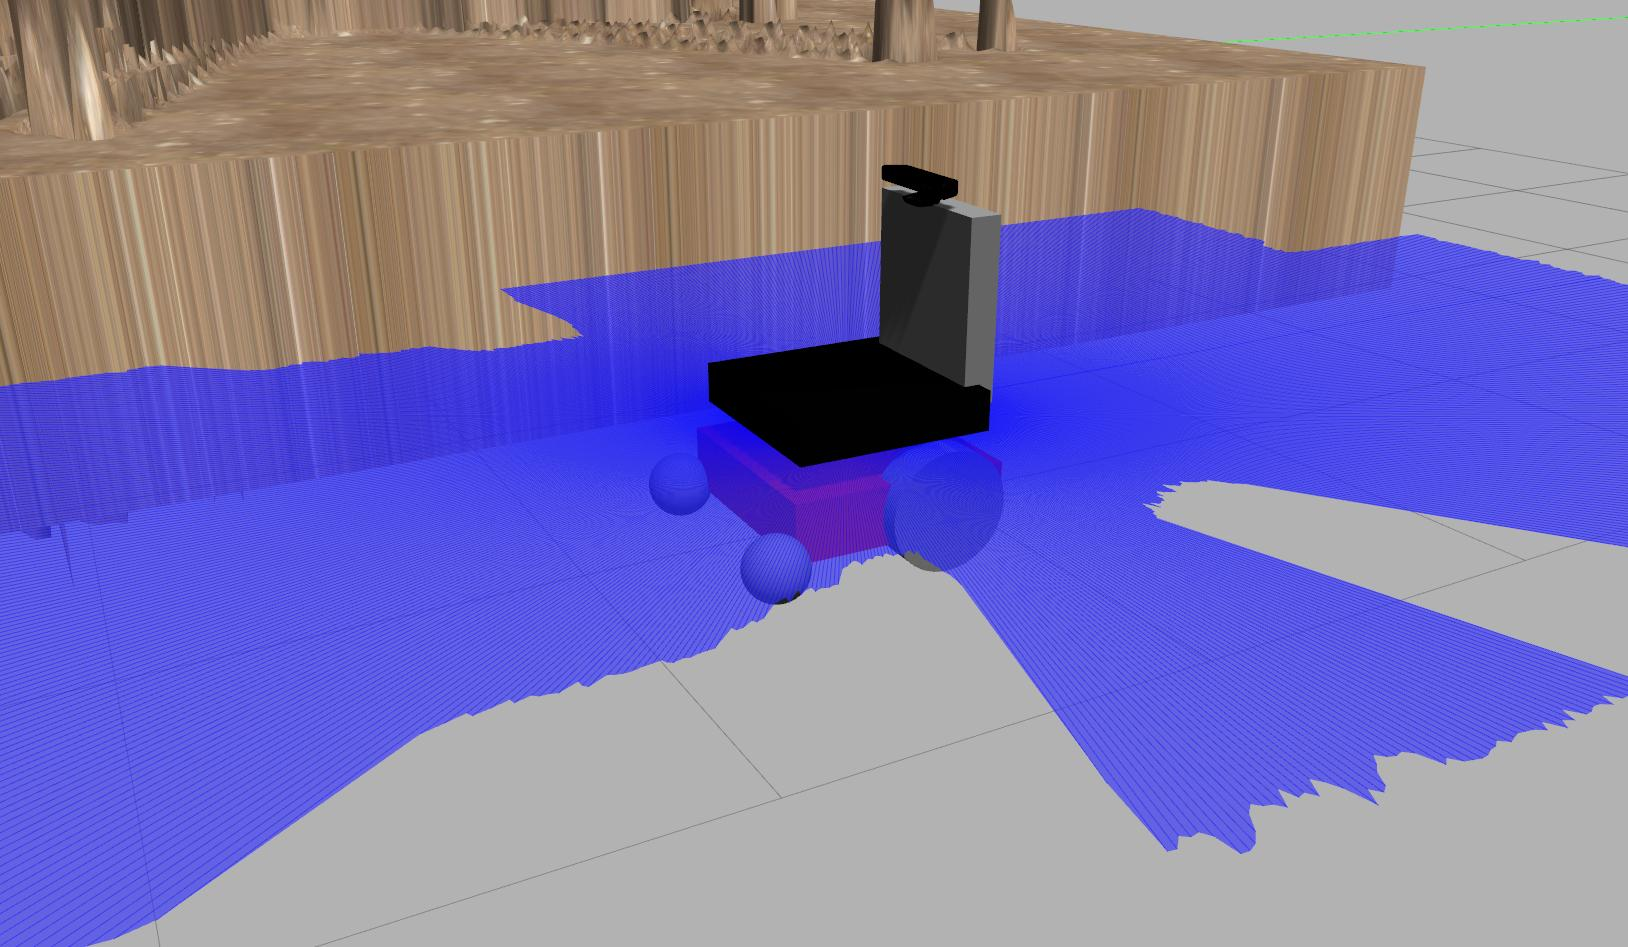
\includegraphics[width=1.0\linewidth]{img/chapter6_test/artamodel.jpg}
		\caption{URDF model of ARTA with joints that model the kinematics of the wheelchair.}
	\end{subfigure}%
	\hspace{\fill} 
	\begin{subfigure}[b]{.48\textwidth}
		\centering
		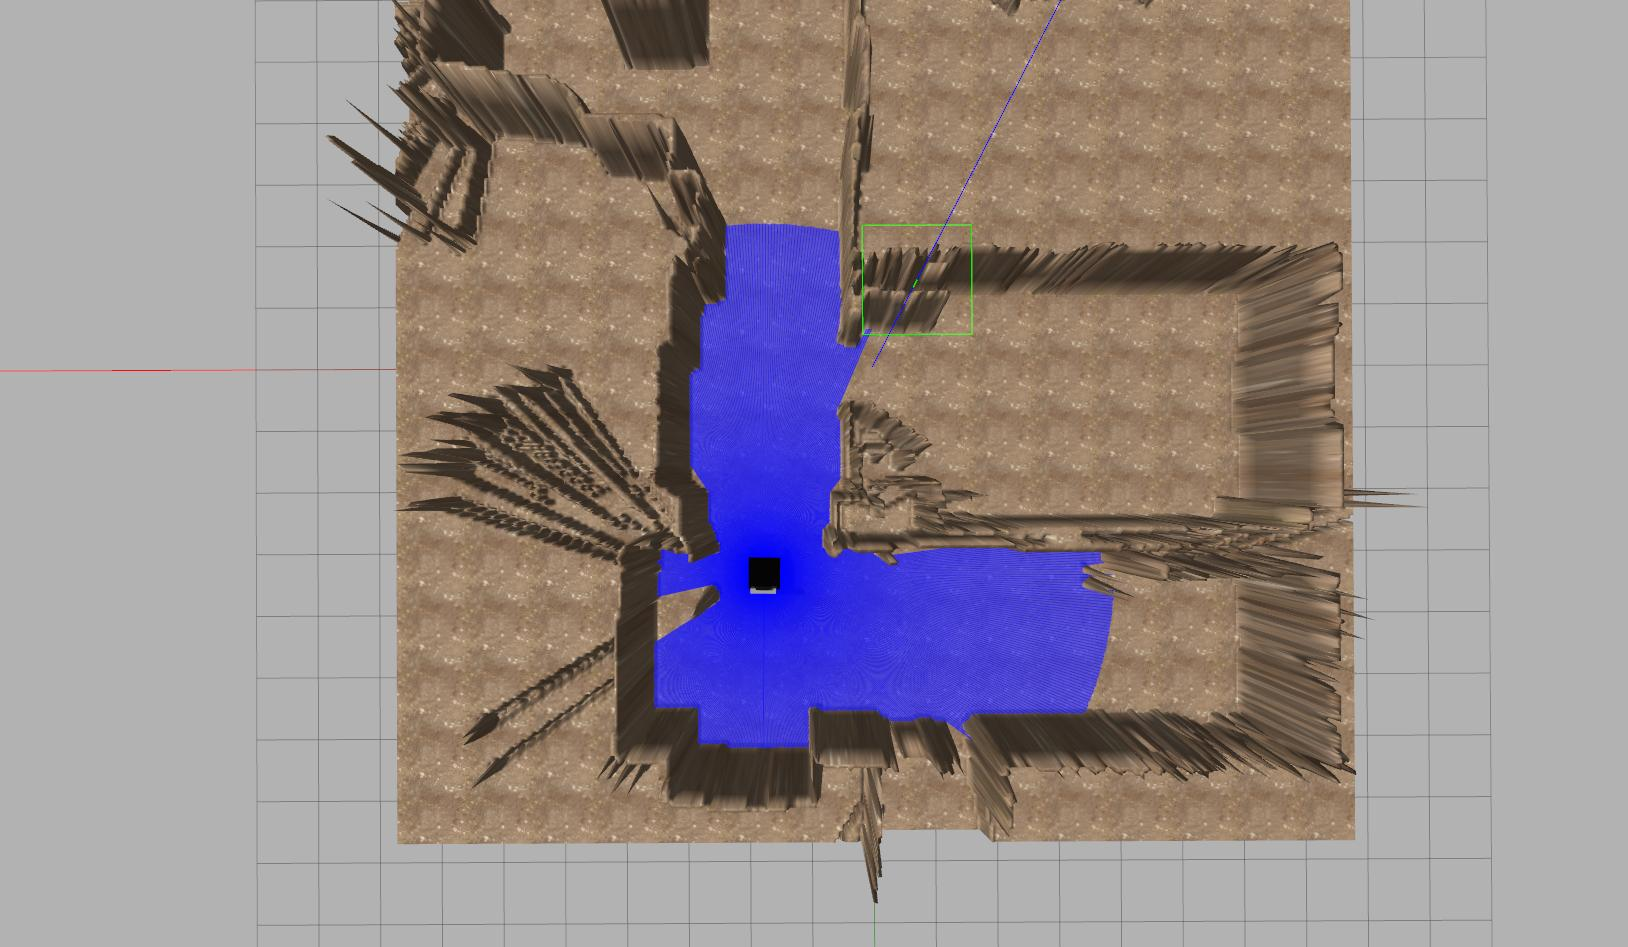
\includegraphics[width=1.0\linewidth]{img/chapter6_test/heightmap.jpg}
		\caption{An aerial view of the Lab Hallway on the 10th floor.}
	\end{subfigure}
	\vspace{-1\baselineskip}
	\begin{center}
		\caption{The Gazebo Simulation of the lab hallway outside the PRL. The blue mesh represents the range of the simulated laser scanner.}
		\label{fig:greenredrender}
	\end{center}
	\vspace{-1\baselineskip}
\end{figure}

\begin{figure}[ht!]
	\begin{subfigure}[b]{.48\textwidth}
		\centering
		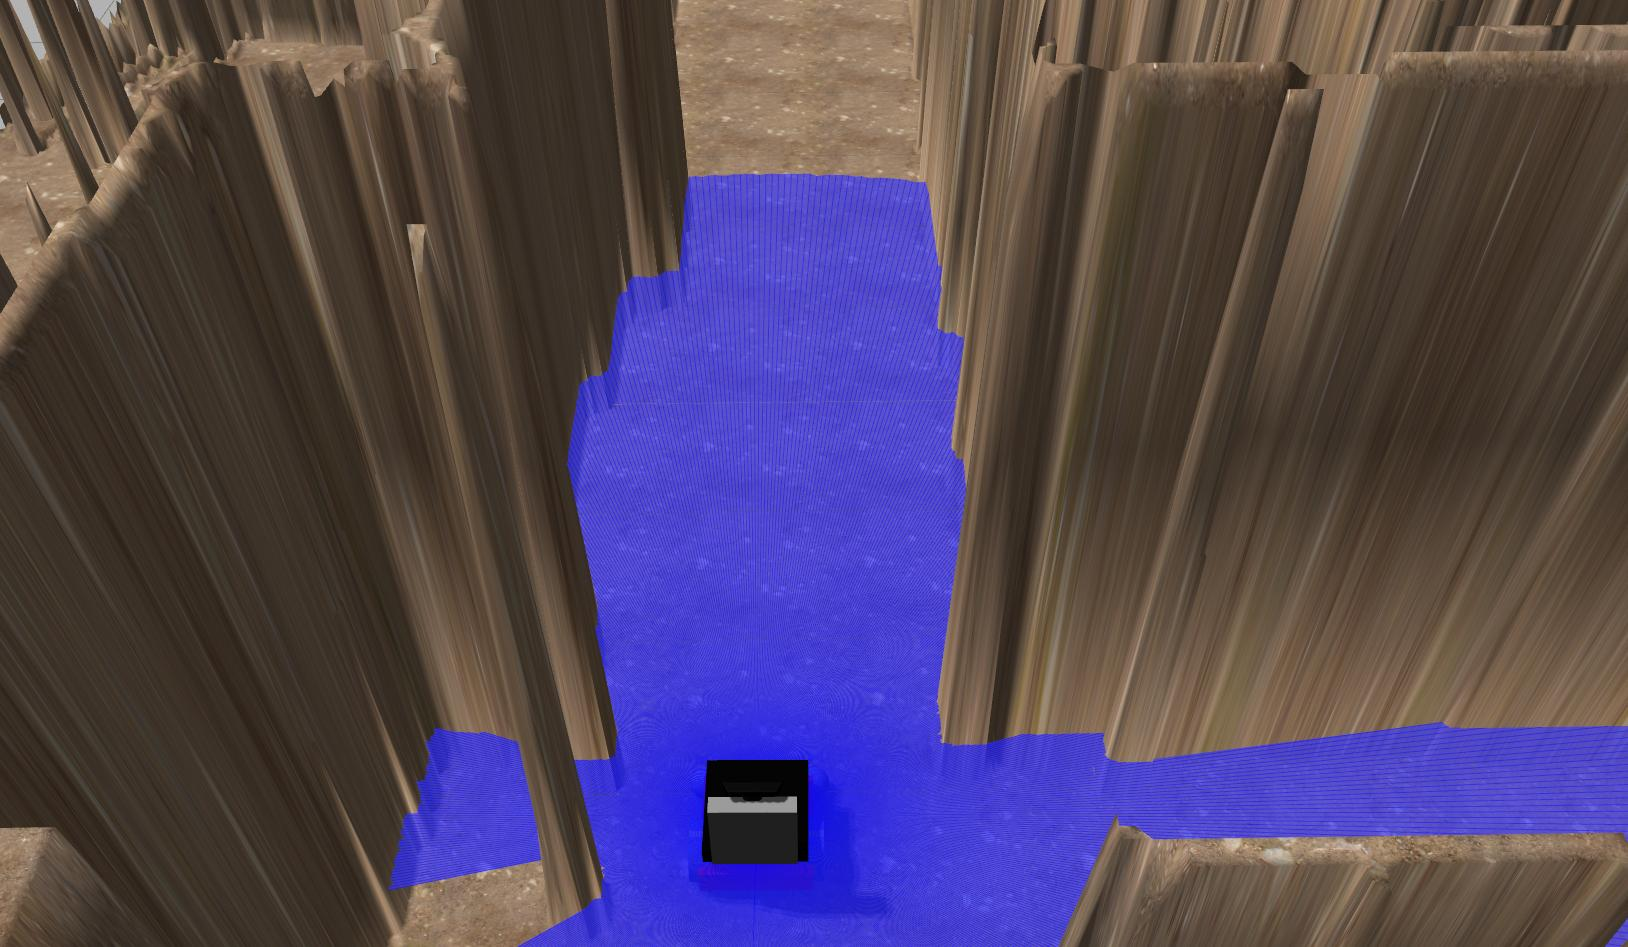
\includegraphics[width=1.0\linewidth]{img/chapter6_test/gazeboBack.jpg}
		\caption{Gazebo Simulation of hallway from behind the model.}
	\end{subfigure}%
	\hspace{\fill} 
	\begin{subfigure}[b]{.48\textwidth}
		\centering
		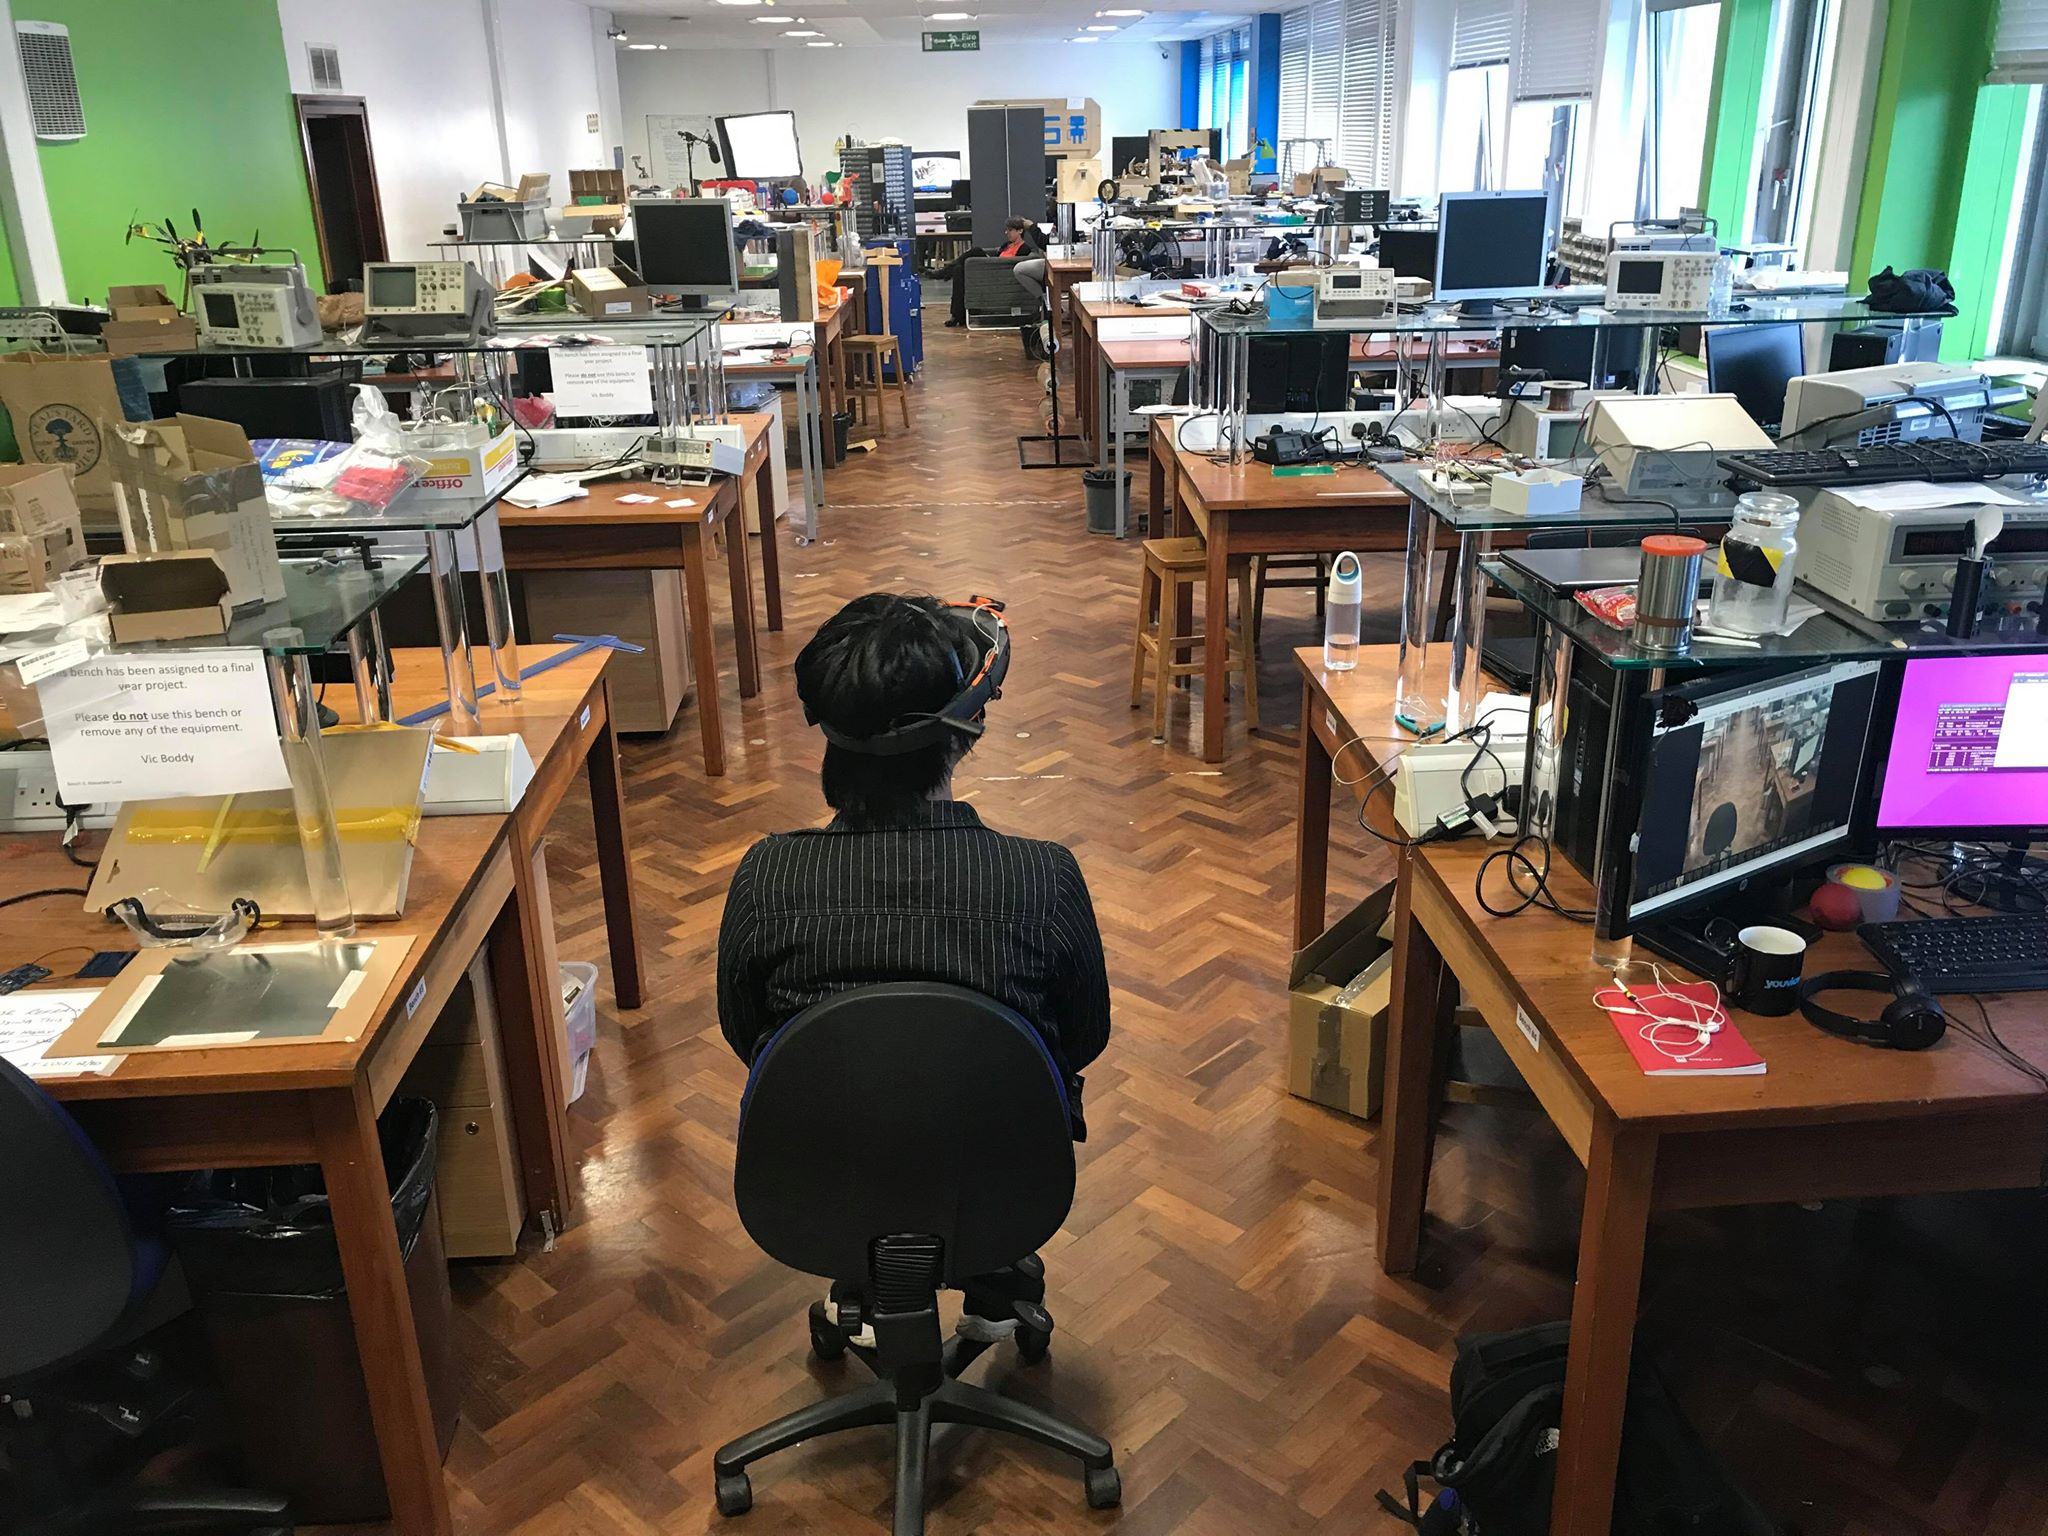
\includegraphics[width=1.0\linewidth,height=41.5mm]{img/chapter6_test/realBack.jpg}
		\caption{Corresponding real world lab setup from behind.}
	\end{subfigure}

	\begin{subfigure}[b]{.48\textwidth}
		\centering
		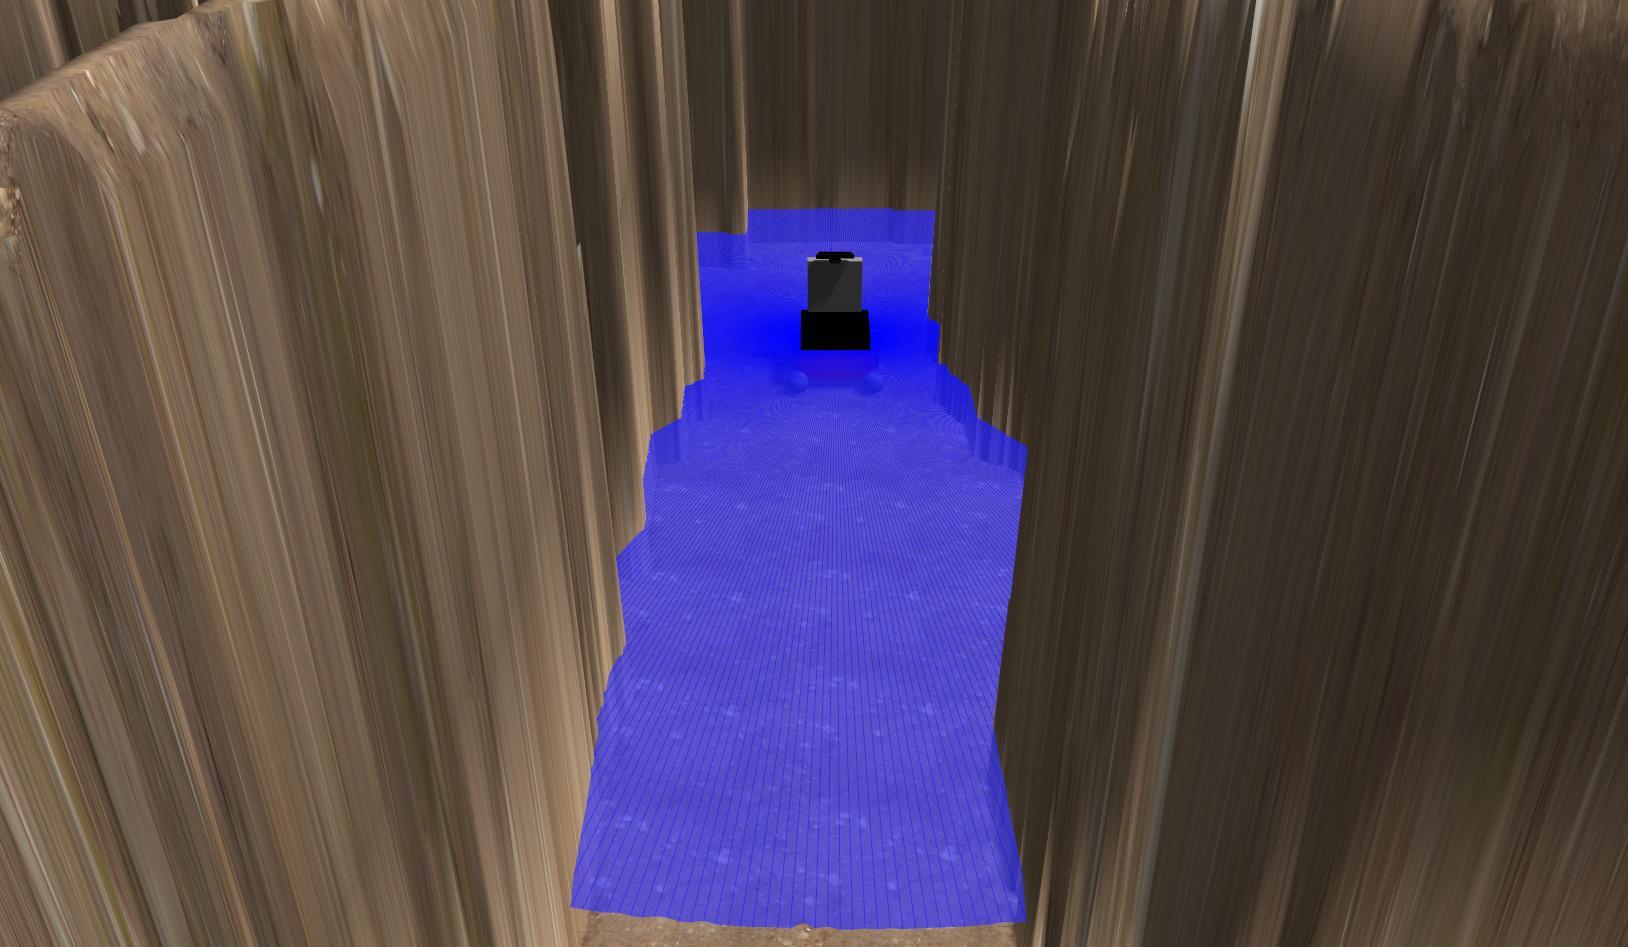
\includegraphics[width=1.0\linewidth]{img/chapter6_test/gazeboFront.jpg}
		\caption{Gazebo Simulation of hallway from in front of the model.}
	\end{subfigure}%
	\hspace{\fill} 
	\begin{subfigure}[b]{.48\textwidth}
		\centering
		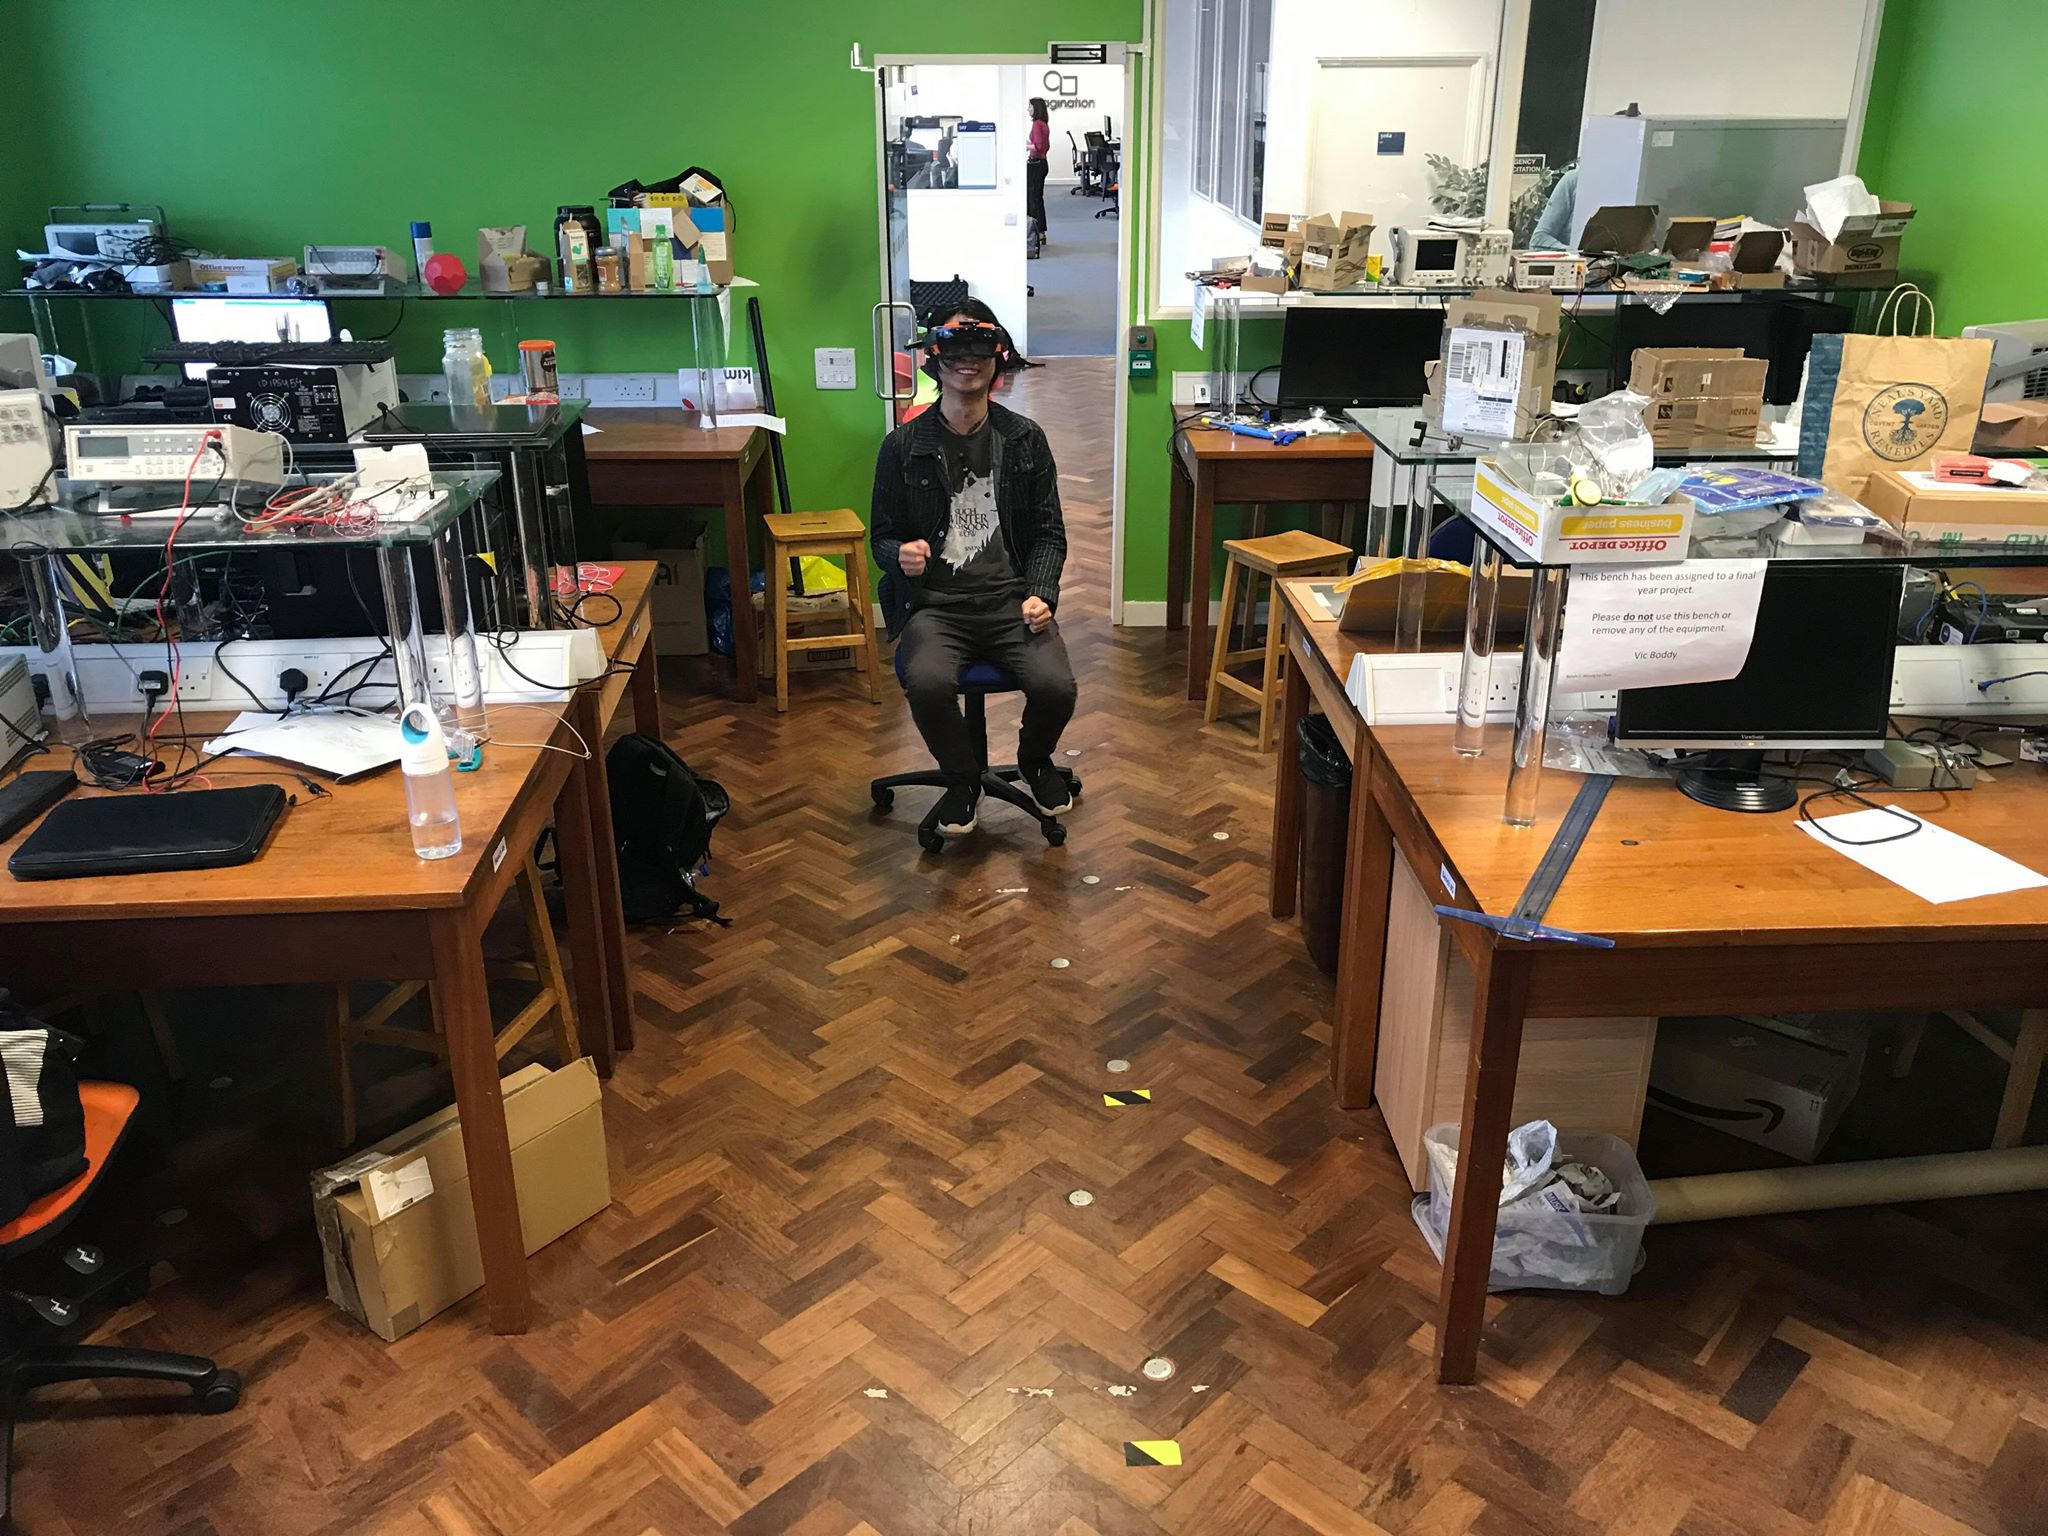
\includegraphics[width=1.0\linewidth,height=41.5mm]{img/chapter6_test/realFront.jpg}
		\caption{Corresponding real world lab setup from in front.}
	\end{subfigure}
	\vspace{-1\baselineskip}
	\begin{center}
		\caption{We emulate the real world position of the Gazebo model position in the ICRS lab. We monitor the simulated velocity of the wheelchair as we vary the distance the target person is from the Hololens.}
		\label{fig:greenredrender}
	\end{center}
	\vspace{-2\baselineskip}
\end{figure}

\subsubsection{Real World Lab Setup}
We are trying to test how the velocity of the wheelchair changes when the system detects a collision risk. We model the movement of the wheelchair in the Gazebo simulation, but we need real human detections to test the reactive control system. We use the same setup used in Section \ref{sec:testSetup}, where we use the long hall between benches in the 5th floor ICRS lab to replicate the hallway outside the PRL lab.

\subsubsection{Monitoring ROS Topics}
We record the ROS topics publishing the linear and angular velocities of the simulated wheelchair using a ROS Bag. We monitor the following topics:

\begin{itemize}
	\item \code{/navigation/main\_js\_cmd\_vel}, the velocity controlled by joystick inputs.
	\item \code{/holo/cmd\_vel}, the reactive control velocity.
	\item \code{/arta/cmd\_vel}, the simulated velocity of the wheelchair.
\end{itemize}

\subsection{Test Procedure}
We asked the test subject to sit in a chair in the middle of the hallway wearing the Hololens. Similar to the experiment in Section \ref{sec:testSetup}, the target person stands at different distances to the test subject. Using the keyboard, we control the simulated wheelchair driving it forward down the simulated hallway. At each marked distance, we  record the joystick, reactive control and final velocities of the simulated wheelchair using the ROS bag for comparison. We test distances between $1$ and $4$ meters away, since the reactive control system only takes over for detections closer than $3$ meters. 

\paragraph{}After the distance tests, the test subjects were asked to look to the side as the simulated wheelchair moved forward. We asked the target person to stand to the side of the wheelchair to provide a human detection. This was done to test if the system can realize the detection is not in the trajectory of the wheelchair, and for the system to realize reactive control is not necessary.

\subsection{Results}
We present the results of this experiment in Figure \ref{fig:reactiveResults}. At a distance of 4 meters, the reactive control was not activated. As such, there is no difference between the joystick input and reactive control velocities, so we omit those results from the figure.

\paragraph{}We note at $3$ meters that the reactive control system detects a collision risk and reacts appropriately by reducing the velocity of the wheelchair. We see in Figure \ref{fig:reactiveResults}.a that the output velocity of the reactive control system is below the ideal reactive control velocity of $0.5$m/s. Furthermore, the velocity oscillates between $0.3$m/s and $0.1$m/s, well below the ideal velocity. Figure \ref{fig:reactiveResults}.b shows a similar trend, whereby the output velocity of the reactive control system is $0$m/s instead of the ideal value of approximately $0.1$m/s in the ideal case. Similarly, Figure \ref{fig:reactiveResults}.c also shows a discrepancy. However, more significantly is that there are oscillations in the velocity caused by flickering detections. 

\begin{figure}[ht]
	\begin{subfigure}[b]{1.0\textwidth}
		\centering
		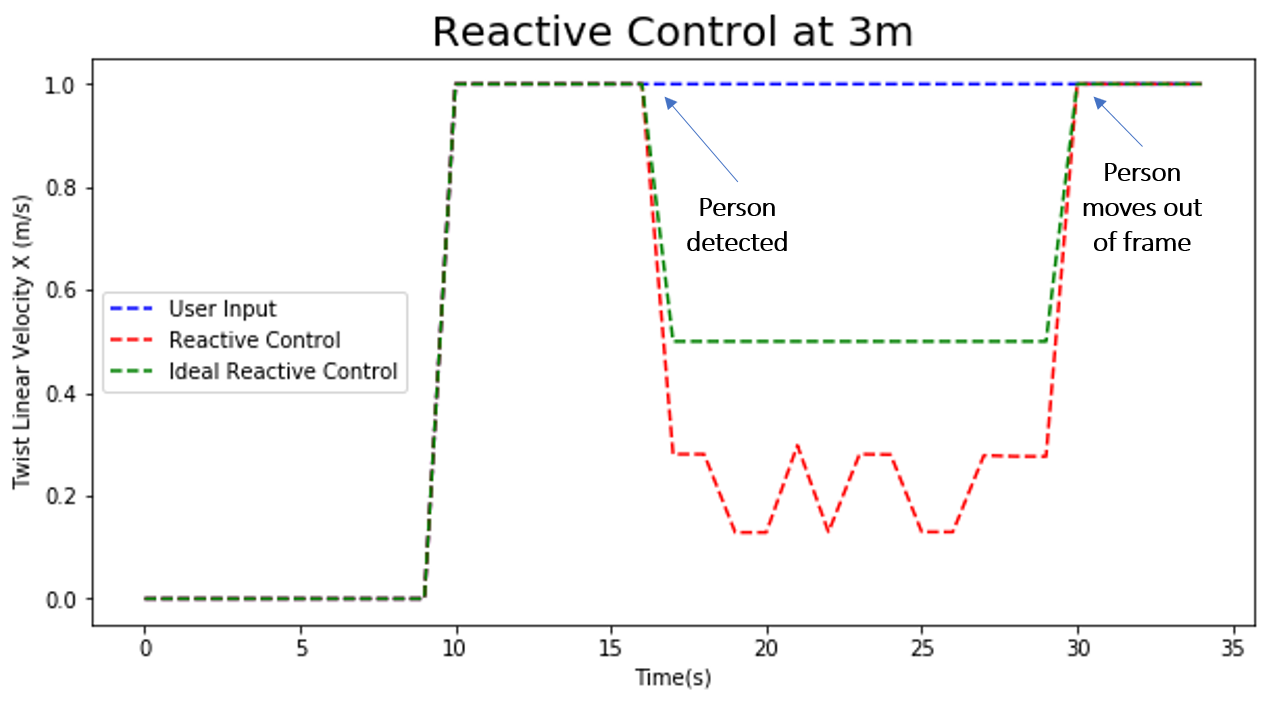
\includegraphics[width=0.75\linewidth]{img/chapter6_test/reactive3.png}
		\caption{Upon detection, the reactive control reduces the velocity to around 0.3m/s. When the collision risk is gone, it returns to 1.0m/s.}
	\end{subfigure}%
	\hspace{\fill} 
	\begin{subfigure}[b]{1.0\textwidth}
		\centering
		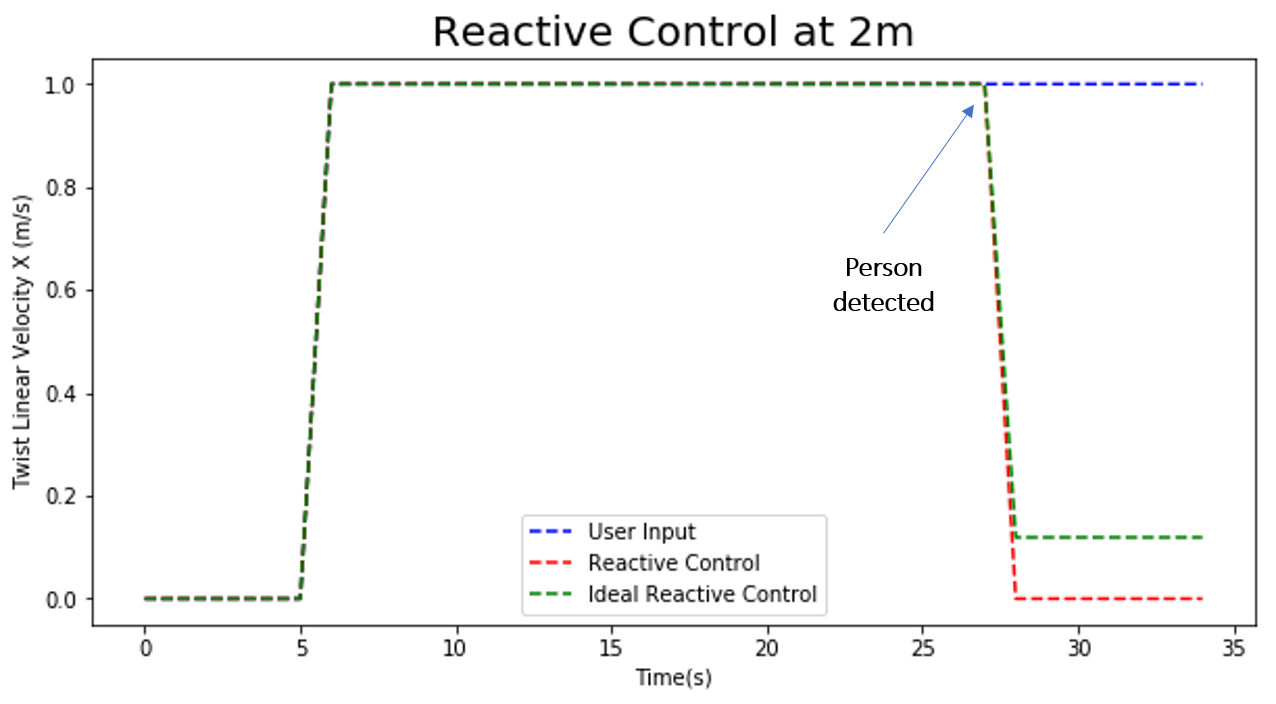
\includegraphics[width=0.75\linewidth]{img/chapter6_test/reactive2.png}
		\caption{At a distance of 2m from the detection, the reactive control system prevents the wheelchair from moving at all.}
	\end{subfigure}
	\begin{subfigure}[b]{1.0\textwidth}
		\centering
		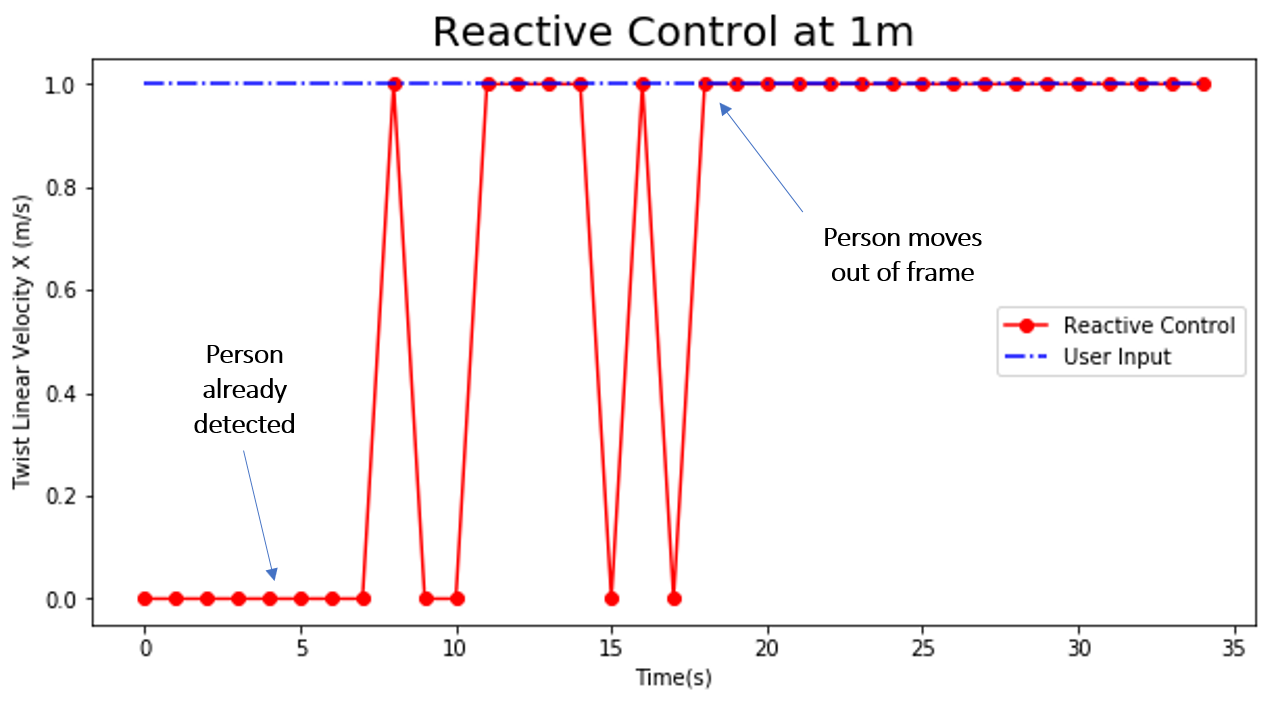
\includegraphics[width=0.75\linewidth]{img/chapter6_test/reactive1.png}
		\caption{The reactive control output velocity oscillates between 0 and 1 due to flickering detections. HDD fails to detect people if they are too close.}
	\end{subfigure}
	\vspace{-1\baselineskip}
	\begin{center}
		\caption{Reactive Control System velocity outputs at different distances.}
		\label{fig:reactiveResults}
	\end{center}
	\vspace{-2\baselineskip}
\end{figure}



%\section{ARTA Reactive Control}